\documentclass[10pt,a4paper]{article}
\usepackage[utf8]{inputenc}
\usepackage{amsmath}
\usepackage{amsfonts}
\usepackage{amssymb}
\usepackage{graphicx}
\usepackage{float}
\graphicspath{{../}}
\usepackage[left=2cm,right=2cm,top=2cm,bottom=2cm]{geometry}
\title{Compton Imaging : CZT-NaI pair}
\begin{document}
\maketitle
\begin{figure}[H]
\centering
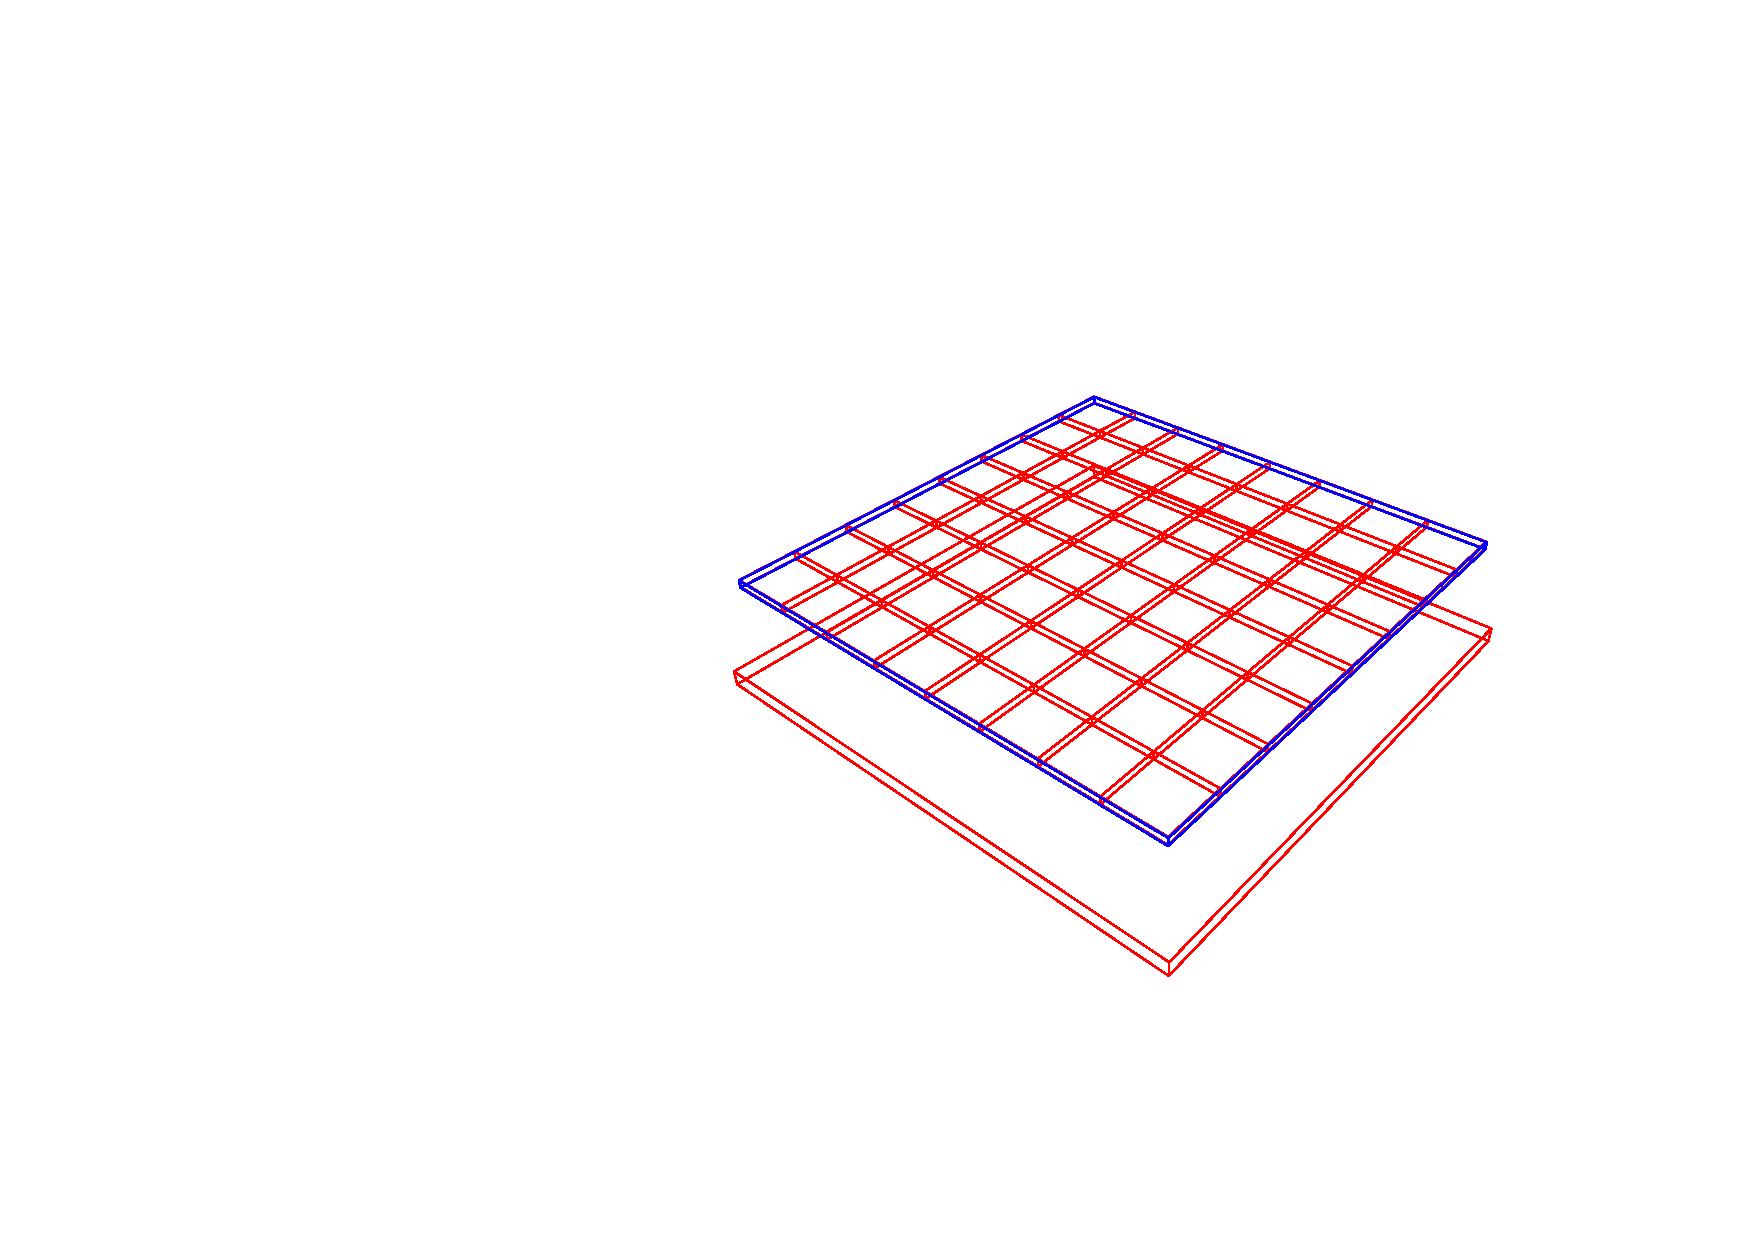
\includegraphics[scale=.75, angle=270, origin=c]{czt_nai_modular}
\end{figure}
The above image shows the geometry built. 64 CZT detector modules, each with dimensions 3.906 cm X 3.906 cm X 0.5 cm were used. Each module contains 256 pixels, making each pixel of size 0.244cm (Different pixel sizes yet to be implemented for the borders). \\
The secondary detector is NaI strip detector, with dimensions 16.7 cm X 16.7 cm X 1 cm . The strip numbers are 20 X 20 .
The gap between the lower surface of CZT and upper surface of NaI is 6.075 cm. 
A monoenergetic source of 600 keV is used. The flux is 5.0 ph/cm$^2$/s, which with a detector area of 976.4 cm$^2$, results in 5000 ph/s .The simulation is run for 100s (observation time). \\
\newpage
\begin{figure}[H]
\centering
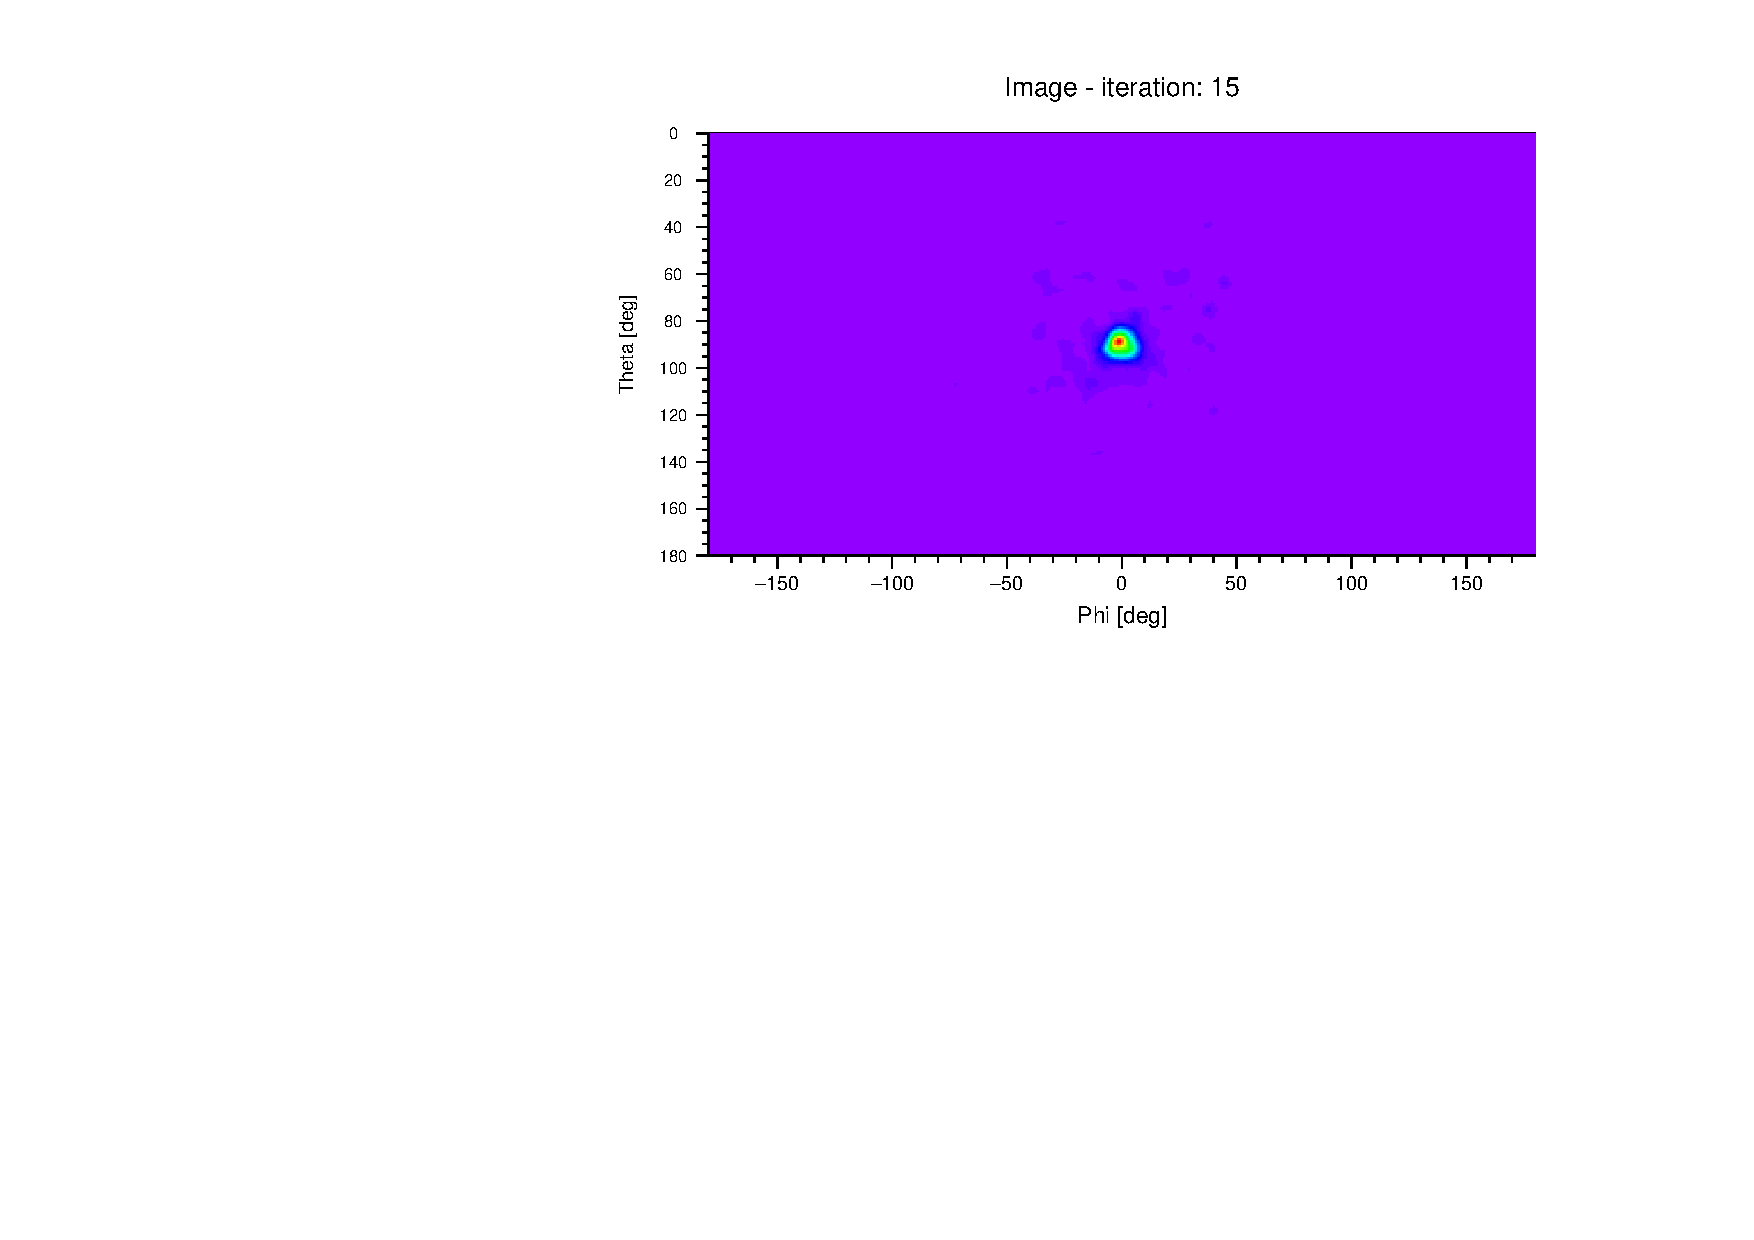
\includegraphics[trim={0 5cm 0 5cm}, scale=.75, angle=270, origin=c]{czt_original}
\caption{Gap between detectors = 6.075cm, Voxel size = 2.44mm, thickness of CZT=0.5cm, Number of Compton Events=19753}
\end{figure}

\begin{figure}[H]
\centering
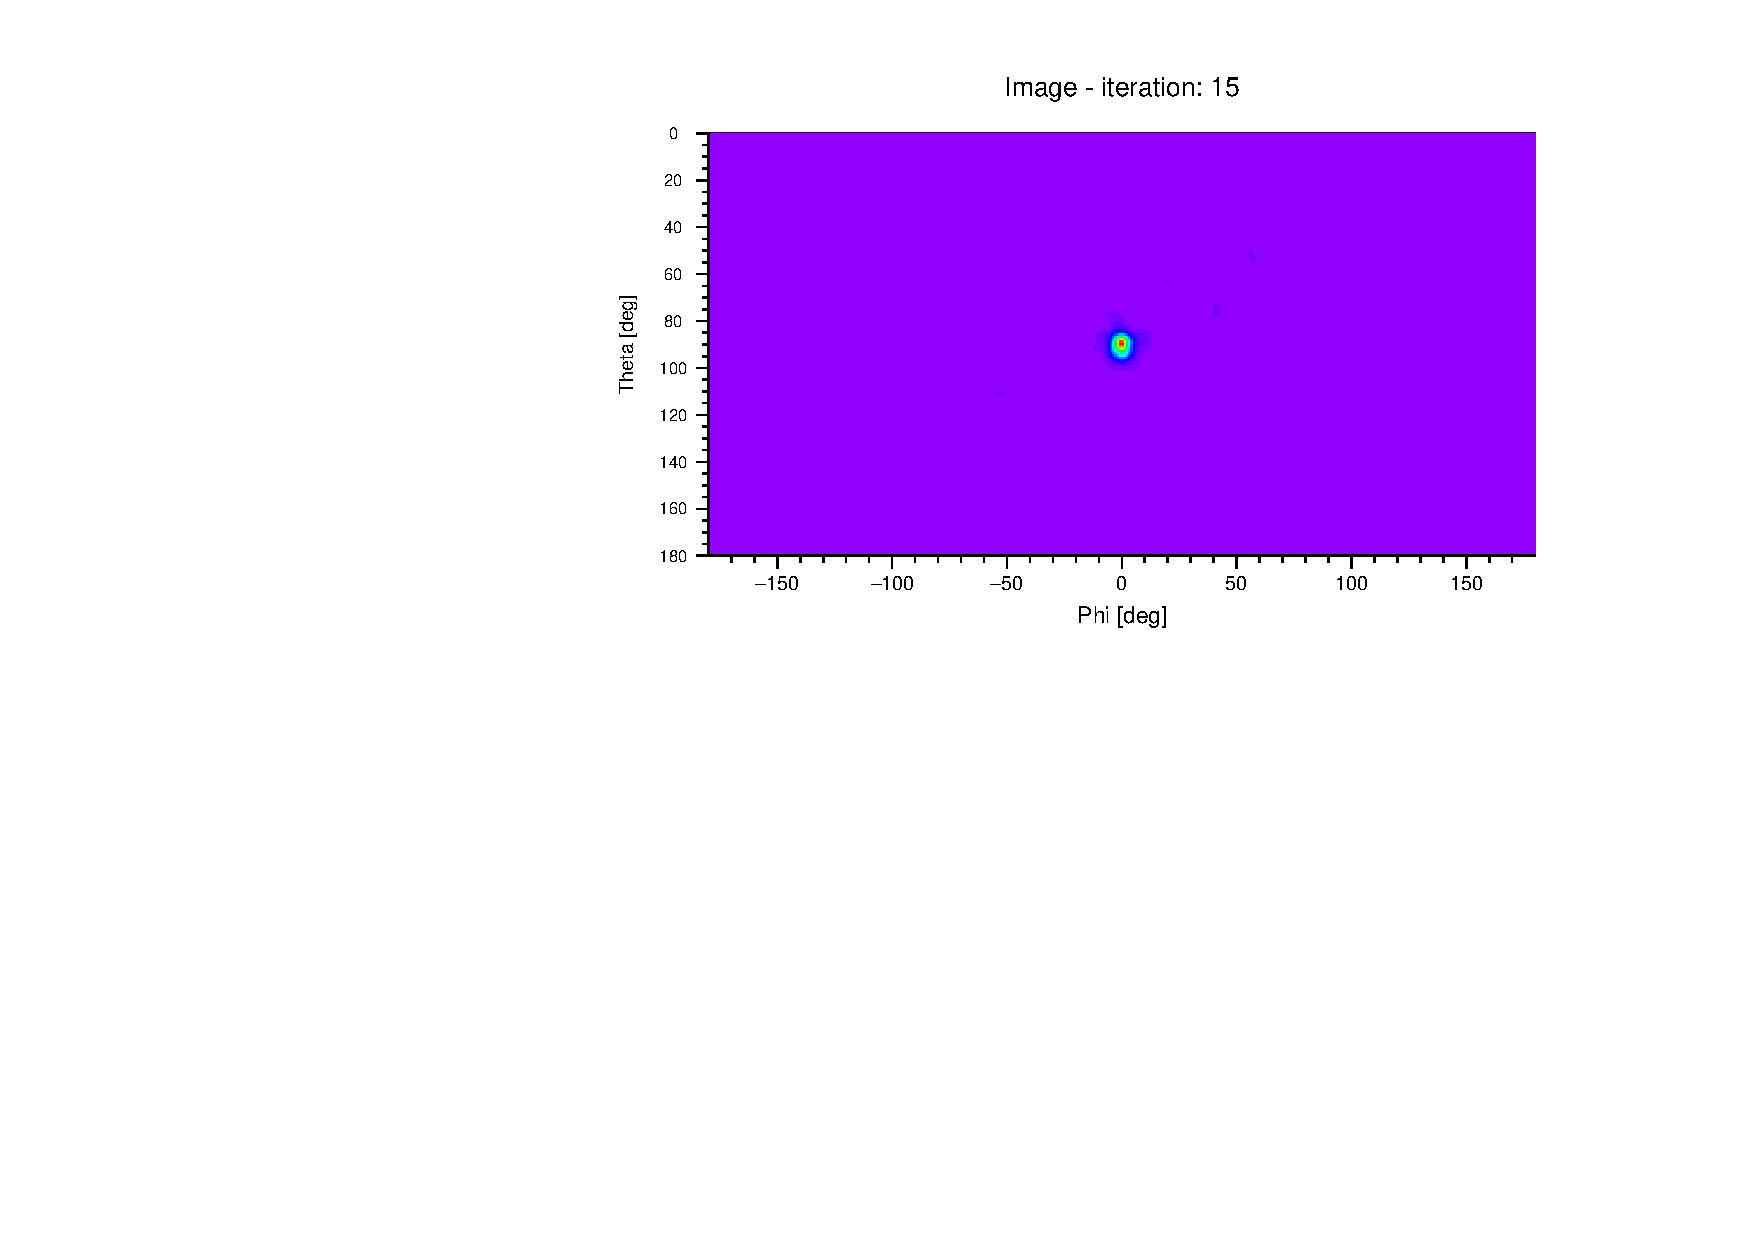
\includegraphics[trim={0 5cm 0 5cm}, scale=.75, angle=270, origin=c]{czt_g12}
\caption{Gap between detectors = \textbf{12cm}, Voxel size = 2.44mm, thickness of CZT=0.5cm, Number of Compton Events=18048}
\end{figure}

\begin{figure}[H]
\centering
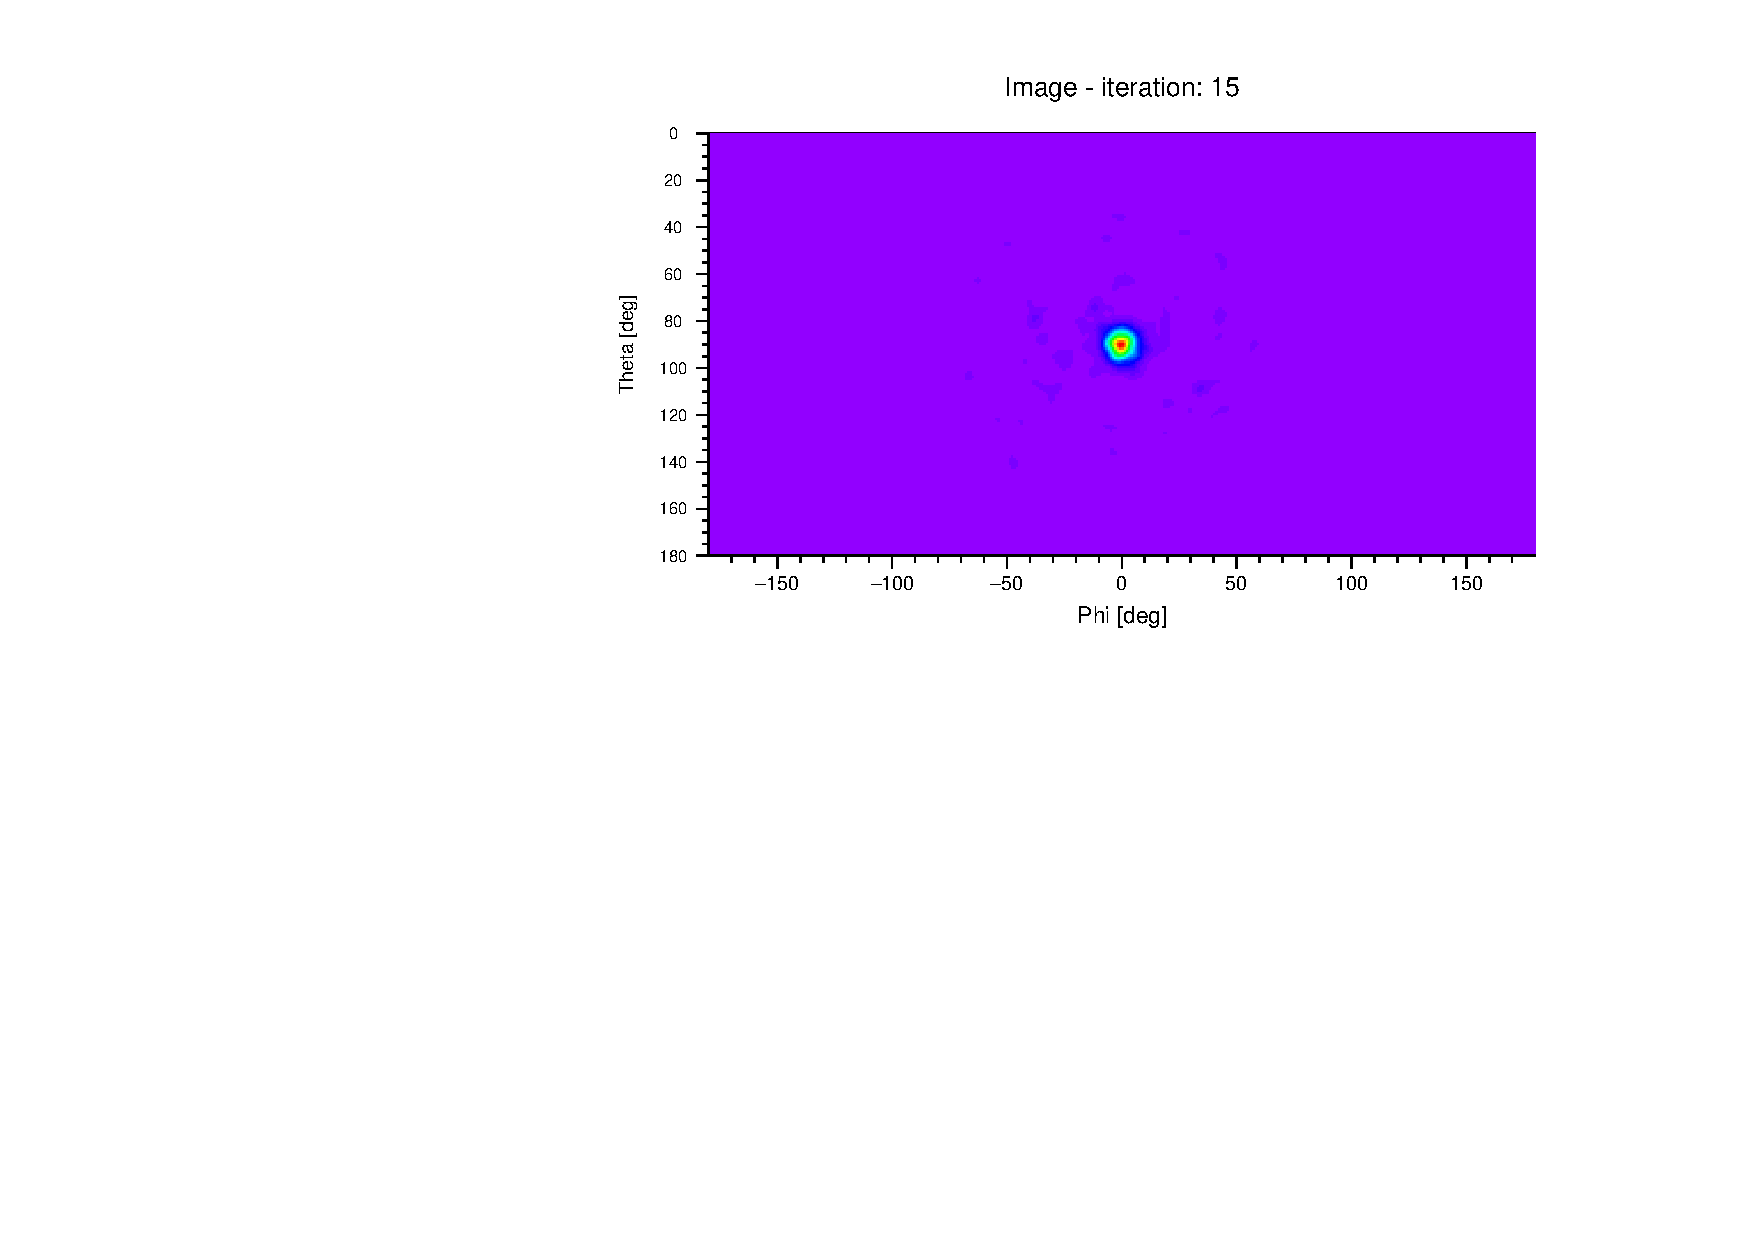
\includegraphics[trim={0 5cm 0 5cm}, scale=.75, angle=270, origin=c]{czt_v0122}
\caption{Gap between detectors = 6.075cm, Voxel size = \textbf{1.22mm}, thickness of CZT=0.5cm, Number of Compton Events=26402}
\end{figure}

\begin{figure}[H]
\centering
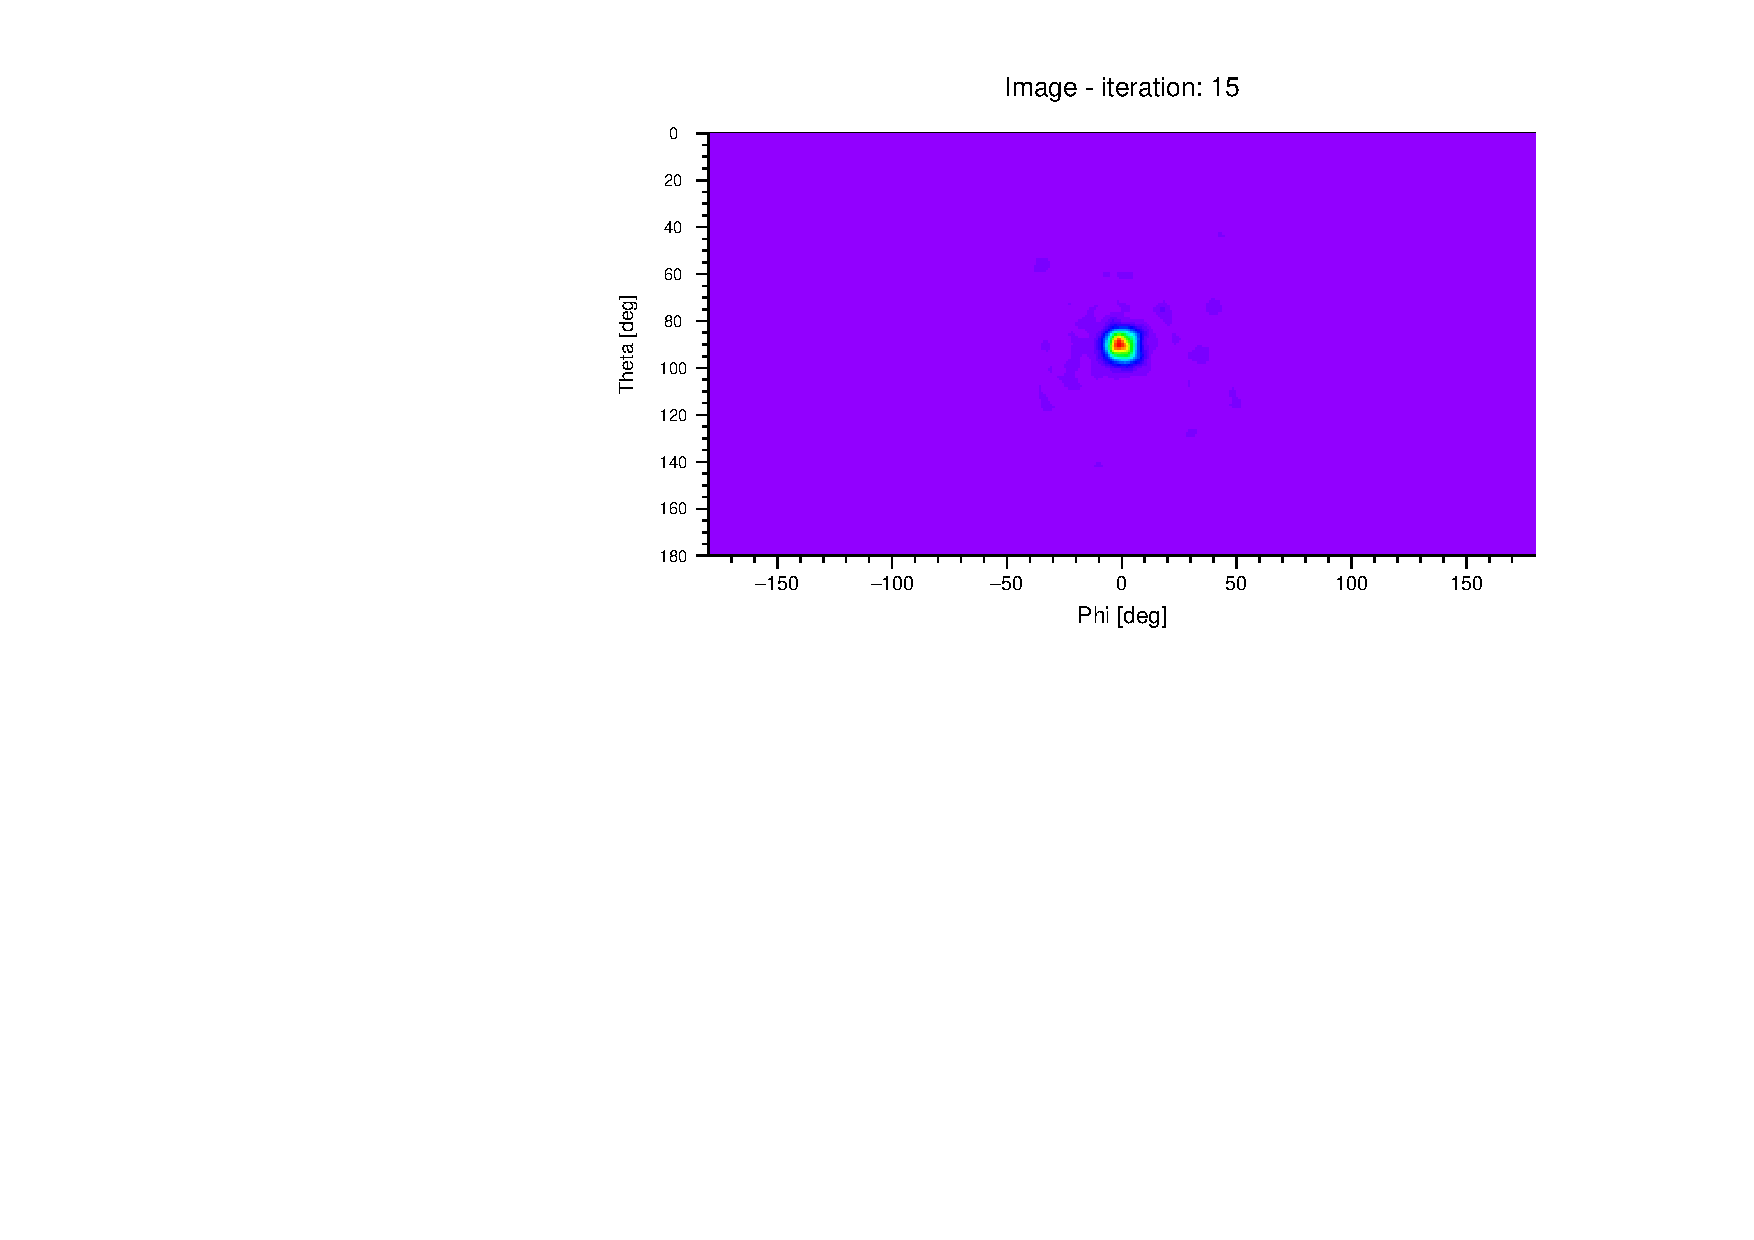
\includegraphics[trim={0 5cm 0 5cm}, scale=.75, angle=270, origin=c]{czt_t_czt_1}
\caption{Gap between detectors = 6.075cm, Voxel size = 2.44mm, thickness of CZT=\textbf{1cm}, Number of Compton Events=27462}
\end{figure}

\end{document}